\chapter{Introduction and Literature Review}

\begin{quote}
  Epoch watch: Welcome to the Sociotechnocene.\\
  -@peterdodds \href{https://twitter.com/peterdodds/status/156899358573465601}{10 Jan 2012}
\end{quote}

\section{Introduction}

%% \sout{Long before the titans of Silicon Valley were disrupting industries with new technology, the widespread use of human language---our great social technology---fundamentally changed our ability to reason and communicate.}
Individual words encapsulate information and emotion as the building blocks that we use to capture experiences in stories.
Beyond words, multi-word expressions (phrases) and complicated grammar coalesce to provide incredible expressive power.
%% (but not without bias).
Attempts to quantify the semantic content of language aim to transform a model of meaning that has proven useful to our own cognitive machinery into something more readily applicable for another purpose (e.g., summarization by a computer).
One such goal is to measure the sentiment expressed in written communication, which is broadly known as sentiment analysis.

In our work, we transfer the emotion of single, isolated words into a one-dimensional happiness measure to build the Hedonometer.
Leveraging the Hedonometer technology and modern computational power, we analyze digitized text with the ultimate goal of understanding stories.
This dissertation proceeds as follows: in this chapter we explore the foundations of sentiment analysis and narrative structure.
In Chapter 2 we benchmark and compare methods for sentiment analysis.
In Chapter 3 we apply these methods and extract dominate emotional arcs from digitized text.
In Chapter 4 I discuss various contributions that I have made to published work throughout my Ph.D.
Finally, in Chapter 5 we offer some concluding remarks.

\section{Sentiment analysis}

%% The earliest work analyzing words can be found in concordances: collections of words
The field of Natural Language Processing (NLP) has been around since the advent of computers, but is growing rapidly alongside computational advances.
While major advances have been made, there remain many open problems.
We focus here on a specific NLP problem, namely understanding the emotional content of language.
We refer to the emotional content in a written text broadly as the sentiment.
In addition to the summaries given in recent review articles \cite{giachanou2016like}, the landscape of tools and technologies is expanding quickly and tackling important challenges.
%% confusing
%% Sentiment is semantic but there are semantics in language beyond sentiment that relate to context and the full meaning.
As we will see, sentiment analysis is a subfield of NLP that can benefit from advancement in other realms of NLP as well (e.g., word sense disambiguation).

Application of sentiment analysis span academia and industry.
Just some of the current uses include predicting elections \cite{tumasjan2010predicting}, predicting product sales \cite{liu2007arsa}, predicting stock market movement \cite{bar2011identifying}, and tracking public opinion \cite{cody2015climate}.
NLP and measures of sentiment are used to analyze consumption of information from the media, and societal level decisions are driven by this flow of public opinion online.
Beyond individual and collective decisions, corporate interests demand an understanding of the public feeling towards their products.



Advances in Artificial Intelligence (AI) have elucidated the distinction between problems that are hard for computers and those that are hard for humans---a difference that is not obvious at the outset.
Sentiment is one such task: understanding the sentiment of our friends and colleagues through informal text is easy for us, but it is hard for algorithms.
As we will see, machine learning (often broadly reffered to as AI) is finding uses in all areas of Natural Language Processing (NLP), including advancing the state-of-the-art in sentiment classification and sentiment dictionary creation.

\subsection{Psychology of emotion}

Many methods in existence aim to detect sentiment one-dimensionally, a range of the emotions that are positive to negative.
While this pragmatic approach proves useful, it is conjectured that there are four \cite{jack2014dynamic}, six \cite{ekman1992argument}, or even eight \cite{plutchik1991emotions} core emotions in humans.
The widely acknowledged six emotions identified by Paul Eckman are:
\begin{itemize}
  \item happy,
  \item surprised,
  \item afraid,
  \item disgusted,
  \item angry,
  \item and sad.
\end{itemize}
In Figures~\ref{fig:ekman} and \ref{fig:plutchik}, visualizations of these emotional dimensions are shown.
While we do not expect that each of these six dimensions are orthogonal (as may be inferred from the Figures), a basis of more than two dimensions is likely necessary to represent the full range of emotion.
Indeed, in Figure~\ref{fig:russell} the theory of \cite{russell1980circumplex} attempts to find the core dimensions of emotion using ``small data''.
Each of these theories expands upon the two dimensions considered further here: happy and sad (positive and negative affect).
More complex emotions can be constructed from combinations of these six.

In addition to emotion, where \textit{valence}, \textit{arousal}, and \textit{dominance} are considered the affective properties of words, the semantic concepts (norms) that are measured include (see ):
\begin{itemize}
  \item \textit{valence},
  \item \textit{arousal},
  \item \textit{concreteness},
  \item \textit{age of acquistion},
  \item and \textit{dominance}.
\end{itemize}
%% \begin{figure}[tbp!]
%%   \centering
%%   \includegraphics[width=0.48\textwidth]{figures/}
%%   \caption[]{
%%   }
%%   \label{fig:}
%% \end{figure}

\begin{figure}[tbp!]
  \centering
  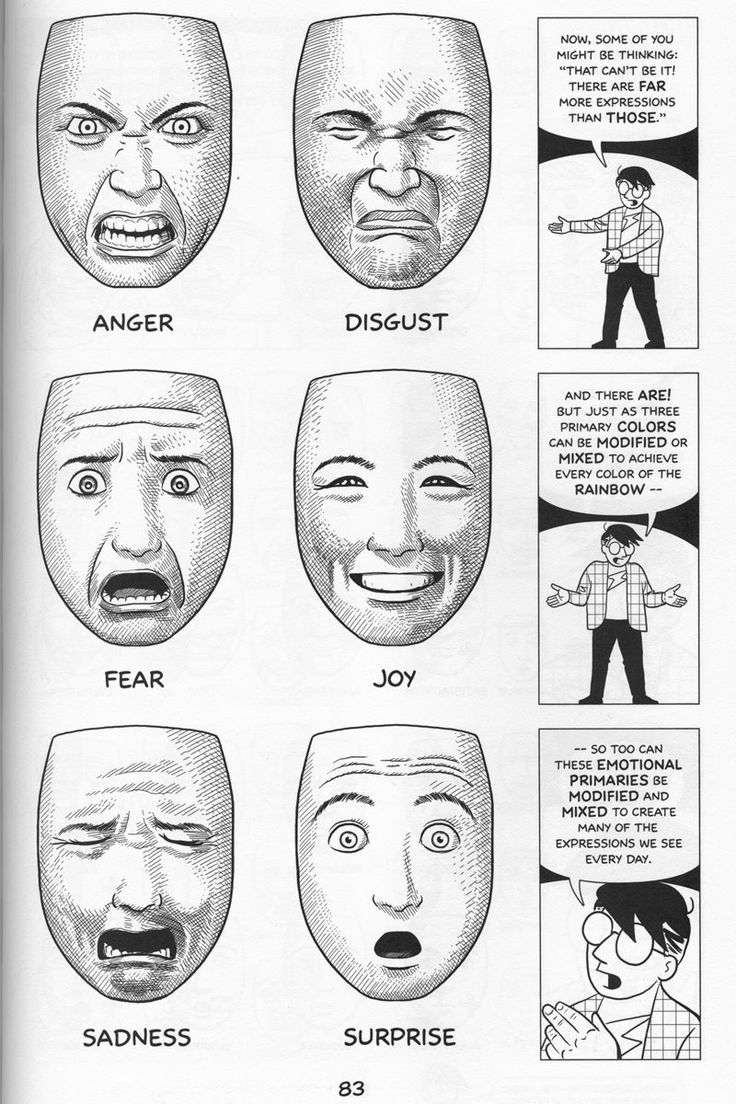
\includegraphics[width=0.48\textwidth]{figures/mccloud.jpg}
  \caption[]{
    The six emotions of \cite{ekman1992argument}, illustrated here by \cite{mccloud2006making}.
    In princple, the entire range of human emotions can be constructed from this minimal ``basis'', e.g., the emotion \textit{delight} is the addition of \textit{joy} and \textit{surprise}.
  }
  \label{fig:ekman}
\end{figure}

\begin{figure}[tbp!]
  \centering
  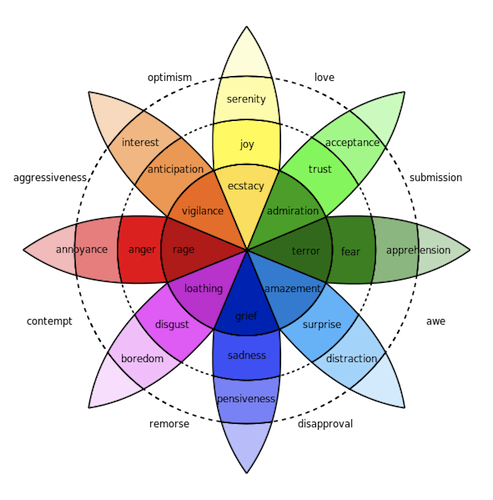
\includegraphics[width=0.48\textwidth]{figures/Plutchik-wheel.png}
  \caption[]{
    Schematic of the eight emotions from \cite{plutchik1991emotions}.
    The commonly known eight names (e.g., joy, etc.) are one row out from the center.
    In addition to the six emotions of \cite{ekman1992argument} we find \textit{anticipation} and \textit{trust}.
  }
  \label{fig:plutchik}
\end{figure}

\begin{figure}[tbp!]
  \centering
  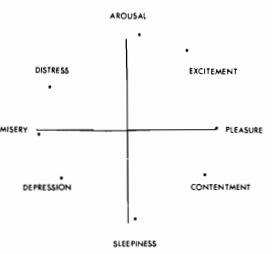
\includegraphics[width=0.48\textwidth]{figures/russell-01.png}
  \caption[]{
    Eight emotions on the arousal--pleasure axis of \cite{russell1980circumplex}, who finds these axis to be the best representation of emotion.
    To this end, using 28 emotional words manually annotated for the characteristics which they share, Russell finds the two major principal components in a PCA analysis, establishing this ``circular ordering.''
  }
  \label{fig:russell}
\end{figure}

For the remainder of this chapter, we will assume that each emotion is being measured on a scale from -1 $\rightarrow$ 1, with 0 representing no presence of emotion and a score of -1/1 representing the maximum negative/positive emotional priming.
While some dictionaries benefit from considering emotion on a different scale for human evaluation (e.g. ``labMT'' with 1 $\rightarrow$ 9 or ``AFINN'' with $-5\to5$), we make this choice to speak more generally about each sentiment dictionary we test.

\clearpage

\subsection{Goals of sentiment analysis}
%% framing of the problem
In general, it may help to first frame the problem of detecting sentiment in text, and next we consider the framing given by Bing Liu in his 2012 book \textit{Sentiment Analysis and Opinion Mining} (see \cite{liu2012sentiment}).
Here, our goal is to detect the average sentiment of a document using the words contained within: \textit{document-level sentiment classification}.
While document length varies, finer-grained analysis can be broken into two categories: classifying sentence-level sentiment and classifying entity-level sentiment.
Sentence-level sentiment is just that, and entity-level sentiment aims to predict sentiments that are directed at named entities (e.g., products, people, or corporations).
We express caution in pursuing these latter goals using existing methodology, namely in classifying short, informal text.
We will examine in Chapter 2 how dictionary based approaches are effective at the document level, but fail at the sentence level.
Several examples of different sentences are also given in \cite{liu2012sentiment}, highlighting the difficulty of classifying individual sentences, and we share these examples here.

Performance is commonly measured using precision, recall, and F-score statistics, as in \cite{ribeiro2016sentibench}.
Next, we review publicly available data sets for sentiment evaluation.

\subsection{Publicly available annotated data}
%% annotation datasets
Review papers such as those by \cite{giachanou2016like} attempt to capture the many advance in the field, including applications of machine learning with training data, though they only find 3 of the 17 sentiment dictionaries that we list in Chapter 2.
%% To address the lack of benchmarks for sentiment analysis on short, informal text, we
They identify the lack of benchmarks are as important issue:
\begin{quote}
  One of the main challenges in evaluating approaches that address Twitter-based sentiment analysis is the absence of benchmark datasets. In the literature, a large number of researchers have used the Twitter API to crawl tweets and create their own datasets, whereas others evaluate their methods on collections that were created by previously reported studies. One major challenge in creating new datasets is how the tweets should be annotated. There are two approaches that have been followed for annotating the tweets according to their polarity: manual annotation and distant supervision.
\end{quote}
%% \todo{Read \cite{tsytsarau2012survey}}
To this end, we note the availability of datasets below and attempt to collect each dataset enumerated by \cite{saif2013evaluation} in Table~\ref{tbl:twitter-data} and make them accessible in one place online.
In addition to these public datasets, some academic groups choose not to release their tagged data, and there are claims of very large datasets held by private companies in the sentiment analysis space.
Given the time and cost associated with obtaining high quality training data, and the ubiquity of machine learning for sentiment analysis in industry, the training data itself is the ``secret sauce'' of these businesses.


\begin{table}
  {\tiny
    
\begin{tabular}{l | l | l | l | l}
  \hline
  Short name & \# Samples & Reference & Citation\\
  \hline
STS,Tweets\_STF,STS-Test & Stanford Twitter Sentiment & 499 & \cite{giachanou2016like,ribeiro2016sentibench,saif2013evaluation}\\
Sanders,Tweets\_SAN,Sanders & Sanders Corpus & 3424 & \cite{giachanou2016like,ribeiro2016sentibench,saif2013evaluation}\\
HCR,HCR & Health Care Reform & 4616 & \cite{speriosu2011twitter}\\
OMD,Tweets\_DBT,OMD & Obama-McCain Debate & 3298 & \cite{giachanou2016like,ribeiro2016sentibench,saif2013evaluation}\\
SS-Tweet,Tweets\_RN\_I,SS-Twitter & SentiStrength Twitter Dataset & 4243 & \cite{giachanou2016like,ribeiro2016sentibench,saif2013evaluation}\\
SemEval,Tweets\_Semeval,SemEval & SemEval Datasets & 6087 & \cite{giachanou2016like,ribeiro2016sentibench,saif2013evaluation}\\
STS-Gold,STS-Gold & STS-Gold & 2036 & \cite{giachanou2016like,saif2013evaluation}\\
DETC,DETC & Dialogue Earth Twitter Corpus & N/A & \cite{giachanou2016like,saif2013evaluation}\\
Tweets\_RND\_IV & aisopos\_ntua & 500 & \cite{ribeiro2016sentibench}\\
Comments\_TED & TED Comments & 839 & \cite{ribeiro2016sentibench}\\
Comments\_BBC & SentiStrength BBC Comments & 1000 & \cite{ribeiro2016sentibench}\\
Comments\_Digg & SentiStrength Digg Comments & 1077 & \cite{ribeiro2016sentibench}\\
Reviews\_I & SentiStrength Myspace Reviews & 1041 & \cite{ribeiro2016sentibench}\\
RW & SentiStrength Runners World Forum & 1046 & \cite{ribeiro2016sentibench}\\
Comments\_YTB & SentiStrength YouTube Comments & 3407 & \cite{ribeiro2016sentibench}\\
Amazon & VADER Amazon Reviews & 3708 & \cite{ribeiro2016sentibench}\\
Reviews\_II & VADER Movie Reviews & 10605 & \cite{ribeiro2016sentibench}\\
Comments\_NYT & VADER NYT Comments & 5190 & \cite{ribeiro2016sentibench}\\
Tweets\_RND\_II & VADER Tweets & 4200 & \cite{ribeiro2016sentibench}\\
Tweets\_RND\_III & ? & 3771 & \cite{ribeiro2016sentibench}\\
ORT & Opinion Retrieval Twitter & 5051 & \cite{luo2012opinion}\\

\end{tabular}
  }
  \caption{Summary of publicly available Twitter datasets tagged with sentiment labels.
  In respect of Twitter's Terms of Service, lists of the Tweet IDs are provided, as well as a script to download the Tweets through Twitter's public API (note some data may not longer be available).}
  \label{tbl:twitter-data}
\end{table}

%% \subsection{Publicly available sentiment dictionaries}
In addition to the tagged datasets above, we attempt to provide a list comprehensive list of sentiment dictionaries in Chapter 2.

\subsection{Dictionary-based approaches}

The most straightforward approaches to measuring sentiment are dictionary-based, relying upon a sentiment dictionary contains the emotions of specific words and/or phrases.
A pragmatic approach to document classification treats each document as a ``bag of words'', wherein order of the words is unimportant and we only concern ourselves with the frequency of occurrence.
%% Given an individual document $T$ and a dictionary of emotive words $w_i$, we can measure the average sentiment of the document by taking the average of the sentiment scores for each appears of the emotive words $w_i$:
%% \begin{equation} h_\text{avg} ^T = \ldots ,\end{equation}
%% where $h_\text{avg}$ is the average happiness of the document $T$.

We aim to understand and evaluate these methods at a human level, and it is intuitive yet deceiving to consider individual sentences.
At the level of individual sentences, the bag of words approach is no longer useful.
One attempt to improve these models for short text is to incorporate rules that are manually encoded to fit a given model for language, relying on the grammatical structure of language.
Such a rule might be to consider negation words such as ``not'' to reverse the polarity of the following sentiment word, such that ``not $w_i$'' would be combined and assigned the score of ``$-w_i$''.
Without standard benchmarks used by researchers who generate sentiment dictionaries, their individual rule choices are difficult to replicate, and we focus on studying the quality of the sentiment dictionary without using any rules.
In this way, our comparisons are clearly relative, as sentence-level classification can be easily enhanced by simple rules (though the ranking of methods is not strongly affected) \cite{hutto2014vader}.

Constructing sentiment dictionaries
Supervised classifier from \cite{esuli2006sentiwordnet} and graph-based label propagation algorithms \cite{rao2009semi}.

\subsection{Machine learning approaches}

Machine learning (ML) approaches to sentiment analysis make explicit use of annotated data to train classifiers.
State-of-the-art unsupervised ML using Neural Network (NN) word representations have proven successful as improving a wide variety of NLP tasks.
Advances that have enabled their success rely upon corpora on the order of billions of words, and implementations that are efficient by making specific choices for network architecture and objective function.

Deep learning: \cite{tang2014coooolll} induced Twitter sentiment lexicons using sentiment-specific word embeddings, obtained via distant supervision.

\subsection{Related Natural Language Processing}

The English All-Words Task \cite{snyder2004english}.
\begin{quote}
  We describe our experience in preparing the sense-tagged corpus used in the English all- words task and we tabulate the scores.
\end{quote}

Architecture for Parsey McParseface:
A Fast and Accurate Dependency Parser using Neural Networks \cite{chen2014fast}.

GAMBL, Genetic Algorithm Optimization of Memory-Based WSD \cite{decadt2004gambl}.
\begin{quote}
  GAMBL is a word expert approach to WSD in which each word expert is trained using memory- based learning. Joint feature selection and algo- rithm parameter optimization are achieved with a genetic algorithm (GA). We use a cascaded classi- fier approach in which the GA optimizes local con- text features and the output of a separate keyword classifier (rather than also optimizing the keyword features together with the local context features). A further innovation on earlier versions of memory- based WSD is the use of grammatical relation and chunk features. This paper presents the architecture of the system briefly, and discusses its performance on the English lexical sample and all words tasks in SENSEVAL-3.
\end{quote}

\cite{akkaya2009subjectivity}

Rules:
\cite{thelwall2012sentiment}
\cite{hutto2014vader}
Negation:
\cite{kiritchenko2014sentiment}
\cite{owoputi2013improved} develop an improved system PoS and tokenization with Twitter (informal text).

\cite{agarwal2011sentiment} analyzed the usefulness of different features for TSA.
\cite{agarwal2011sentiment} proposed a feature-based model and performed a comprehensive set of experiments to examine the usefulness of various features, including POS and lexicon features.
The analysis showed that the most useful combination is the one of POS with the polarity of words.
\cite{kouloumpis2011twitter}

\subsection{Building corpus specific sentiment dictionaries}

\input{\filenamebase.paper04}

\subsection{Scalability}

Using the straightforward dictionary-based average, we are able to process 100 million Tweets per day to serve the online, interactive time series of happiness for the Twitter gardenhose feed at \url{http://hedonometer.org}.
The tweets are processed slightly faster than real time, with fours job running simultaneously on the Vermont Advanced Computing Core (VACC) every hour which take approximately 10 minutes to complete, each processing 15 minutes of Tweets from the previous hour.
We choose to update the time series with daily averages, a time scale that provides enough data to filter out noisy signals while still showcasing a regular weekly pattern.
This ``data mining'' is possible using hash-based dictionary lookups for sentiment scores for each word, and simple word tokenization of the Tweet text.
We aggregate the scores for each 15 minutes into a word vector that represents the count of each word in the labMT sentiment dictionary, sorted by happiness.
In addition to saving these word vectors, we also save a pickled version of the raw word-count hash table for all tokenized words appearing in the 15 minutes.

Using 100 concurrent processes (more will over-saturate the network from file transfers with the IBM GPFS) we are able to search all tweets using the above methodology in less than two days.
The entire database, approximately 370TB uncompressed, could be searched more efficiently by utilizing file storage schemas which localize files to eliminate networked file transfers.
We estimate that a localized file system would allow linear scaling of the search, such that a full database search using the entire VACC would take on the order of 1 hour, by utilizing all 1896 processors across 152 nodes.
More complicated rules for sentiment classification can only serve to slow the overall speed.
As we investigate in greater detail in Chapter 2, some dictionaries employ word stems, which make the lookup between 10 and 1000 times slower.

Machine learning techniques posses the advantage of to classify quickly after the training process.
While it may take days, weeks, or even months to train a deep neural network, look-ups require very little added computational burden.

\subsection{Visualization}

Lacking from the bulk of research that applies sentiment analysis, but crucial for validation and understanding, is visualization of sentiment analysis classification.
Of particular interest for our choice of dictionary-based methods is that straightforward averaging procedure allows for the comparison of text sentiment classification, both enabling greater understanding and validating the most important words.
On a sentence level, we can see without added visual clues which individual words have either positive or negative scores, and how their balance contributes to the average-based classification.
When rules become involved, this process is more complicated and it may be necessary to utilize a sentence diagram to understand the classification at even the individual sentence level.
Neither of these approaches scale to visualize more than individual sentences, a fundamental shortcoming when the question at hands seeks to understand why many million sentences differ from many others.

\begin{figure}[tbp!]
  \centering
  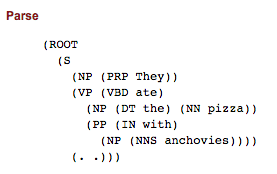
\includegraphics[width=0.48\textwidth]{figures/stanford-1.png}
  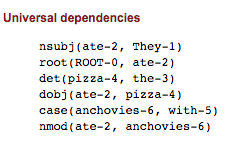
\includegraphics[width=0.48\textwidth]{figures/stanford-2.png}
  \caption[]{
    \cite{chen2014fast}
  }
  \label{fig:}
\end{figure}

\begin{figure}[tbp!]
  \centering
  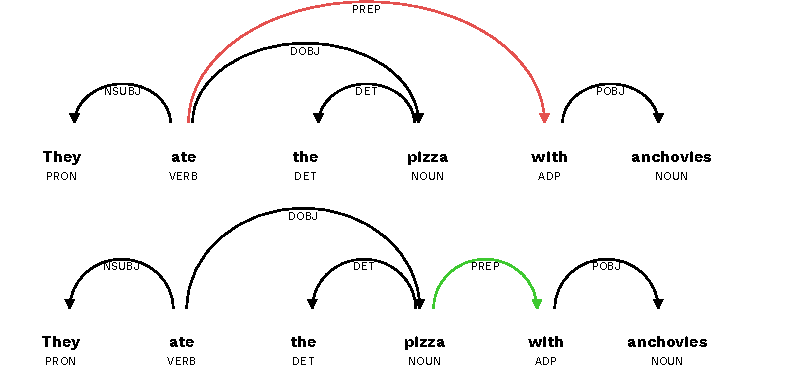
\includegraphics[width=0.48\textwidth]{figures/displacy-both.pdf}
  \caption[]{
    \cite{honnibal2015displaying}
  }
  \label{fig:}
\end{figure}

\begin{figure}[tbp!]
  \centering
  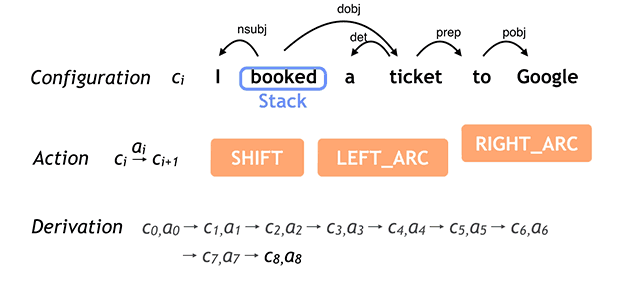
\includegraphics[width=0.48\textwidth]{figures/google-1.png}
  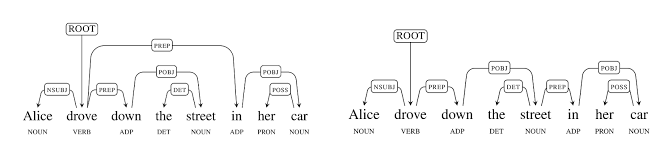
\includegraphics[width=0.48\textwidth]{figures/google-3.png}
  \caption[]{
    \cite{andor2016globally}
  }
  \label{fig:}
\end{figure}

\subsection{Benchmarking literature}

%% here let's try to include papers that really are attempts at benchmarks, in lit review fashions
In this section we review recent efforts to benchmark sentiment analysis methods for their performance.\\

\cite{pang2008opinion}
To quote from \cite{pang2008opinion}, ``\cite{pang2008opinion} provide a comprehensive overview of the SA approaches using various types of data. However, this survey was published some time ago and does not cover recent developments and trends in the field.''
\cite{liu2012survey}

%% \bibentry{liu2012sentiment}
%% this is the book
\noindent \textbf{Liu, B. (2012, May).
{\em Sentiment analysis and opinion mining}.
Synthesis Lectures on Human Language Technologies. San Rafael, CA:
Morgan \& Claypool Publishers.}

This book from Bing Liu provides a broad overview sentiment analysis, and the many different problems that it hopes to address as well as summaries of many common approaches.
Liu provides a framework to understand the aspects of sentiment analysis, with a the varying levels of analysis (aspect, sentence, document level), and goals including classification and opinion summarization.
In Chapter 8, a discussions of the methods for generating sentiment dictionaries is presented, and includes manual, dictionary-based, and corpus based approaches.
Survey methods are not considered (the well-known ANEW dictionary is absent), and there is some confusion between methods that use a dictionary to propogate scores and those that use features of a corpus to propogate scores (\cite{velikovich2010viability} incorrectly classified as the former).
While the references are extensive, no analysis is conducted to understand how the different approaches for generating sentiment dictionaries perform.
Despite these shortcomings, the book is a broad and very useful guide to the landscape of sentiment analysis.

\cite{tsytsarau2012survey}

%% \bibentry{hutto2014vader}
\noindent \textbf{Hutto, C.~J. and E.~Gilbert (2014).
Vader: A parsimonious rule-based model for sentiment analysis of
  social media text.
In {\em Eighth International AAAI Conference on Weblogs and Social
  Media}.}

This paper is focused on the development of a new dictionary-based method for sentiment analysis that incorporates a rule-based system and a dictionary tailored to social media.
While other papers that introduce dictionaries for sentiment analysis have made comparisons between methods (e.g., LIWC correlations between the 2001, 2007, and 2015 dictionaries on their website), we include this as a benchmark because of the uncommon rigor in the comparisons made.
In particular, Hutto and Gilbert compare their new method VADER to 11 other sentiment analysis methodologies.
They compare to seven dictionary-based methods and four ML methods, and find favorable correlations between the classification of Tweets for the dictionary based methods.
In addition they perform tests to measure the performance gains to be had using four rules, and word sense disambiguation, finding mean F1 performance gains of 2 points on individual Tweets.
These rules are a subset of those employed by \cite{thelwall2012sentiment}.
The comparisons between sentiment dictionaries focus on the classification performance, and do not provide any insight into what properties of the dictionaries contributes to their performance.
In addition, no effort is made to use sentiment analysis as more than a binary classifer, a shortcoming that we will address.\\

%% \bibentry{giachanou2016like}
\noindent \textbf{Giachanou, A. and F.~Crestani (2016, June).
Like it or not: A survey of twitter sentiment analysis methods.
{\em ACM Comput. Surv.\/}~{\em 49\/}(2), 28:1--28:41.}

This extensive survey from Giachanou \etal provides an overview and categorization of methods used to quantify sentiment on Twitter.
and no quantitative comparisons are made between the methods themselves.
The broad categories of the methods they find are based on those from \cite{liu2012sentiment}:
\begin{itemize}
\item Machine Learning.
\item Lexicon-Based.
\item Hybrid (Machine Learning \& Lexicon-Based).
\item Graph-Based.
\end{itemize}
The focus is on ML approaches (as they note: ``The majority of [Twitter Sentiment Analysis] methods use a method from the field of machine learning'').\\

%% \bibentry{ribeiro2016sentibench}
\noindent \textbf{Ribeiro, F.~N., M.~Ara{\'u}jo, P.~Gon{\c{c}}alves,
  M.~Andr{\'e}~Gon{\c{c}}alves, and F.~Benevenuto (2016, jul).
{SentiBench} --- a benchmark comparison of state-of-the-practice
  sentiment analysis methods.
  {\em {EPJ} Data Sci.\/}~{\em 5\/}(1), 23.}

This recent benchmark from Ribeiro \etal was published while our work was under review, having been submitted after our preprint was released on the arXiv.
%% submitted Feb 03 from them
The comparisons made by Ribeiro \etal utilize a variety of methods, and provide measures of performance for all methods based on F1 scores.
The methods selected include commerical, ML, and dictionary-based, and they are applied for four corpora.
Beyond metrics of classification performance, no insight is provided into the reasons why certain methods out-perform others, nor is any focus on understanding texts through sentiment (or using visualization), the key tenets of our effort in Chapter 2.

\cite{rosenthal2015semeval}

%%%%%%%%%%%%%%%%%%%%%%%%%%%%%%%%%%%%%%%%%%%%%%%%%%%%%%%%%%%%%%%%%%%%%%%%%%%%%%%%

%%%%%%%%%%%%%%%%%%%%%%%%%%%%%%%%%%%%%%%%%%%%%%%%%%%%%%%%%%%%%%%%%%%%%%%%%%%%%%%%

%%%%%%%%%%%%%%%%%%%%%%%%%%%%%%%%%%%%%%%%%%%%%%%%%%%%%%%%%%%%%%%%%%%%%%%%%%%%%%%%

%%%%%%%%%%%%%%%%%%%%%%%%%%%%%%%%%%%%%%%%%%%%%%%%%%%%%%%%%%%%%%%%%%%%%%%%%%%%%%%%

\section{Emotional arcs}

Stories provide a useful framing to condense our experience, and through this they are both ubiquitous and powerful.
In 2011, a DARPA initiative ``Narrative Networks'' (see \cite{darpa2011narrative}) said the following in relation to security:
\begin{quote}
  Narratives exert a powerful influence on human thoughts and behavior.
  They consolidate memory, shape emotions, cue heuristics and biases in judgment, influence in-group/out-group distinctions, and may affect the fundamental contents of personal identity.
  It comes as no surprise that because of these influences stories are important in security contexts: for example, they change the course of insurgencies, frame negotiations, play a role in political radicalization, influence the methods and goals of violent social movements, and likely play a role in clinical conditions important to the military such as post-traumatic stress disorder.
\end{quote}
%% Secular experiences are the raw matter, the stuff, of our existence.
%% Chains of experiences, or events, are stories.
%% No one wants to watch the every day truman show (but they also do)

The ubiquitous nature of stories is summed up well in \cite{dodds2013homo}:
\begin{quote}
We humans are storytelling and story-finding machines: \textit{homo narrativus}, if you will.
In making sense of the world, we look for the shapes of meaningful narratives in everything.
Even in science, we enjoy mathematical equations and algorithms because they are a kind of universal story.
Fluids---the oceans and atmosphere, the blood in your body, honey---all flow according to a single, beautiful set of equations called the Navier-Stokes equations.

In our everyday, human stories, far away from science, we have a limited (if generous) capacity to entertain randomness---we are certainly not \textit{homo probabilisticus}.
Too many coincidences in a movie or book will render it unbelievable and unpalatable.
We would think to ourselves, ``that would never happen in real life!''
This skews our stories. We tend to find or create story threads where there are none.
While it can sometimes be useful to err on the side of causality, the fact remains that our tendency toward teleological explanations often oversteps the evidence.
\end{quote}

%% dan harmon

%% http://channel101.wikia.com/wiki/File:HeroCycle-Campbell.png

In Chapter 3 we consider previous work that finds between one and 36 different plot types: \cite{campbell2008hero,harris1959basic,abbott2008cambridge,booker2006seven,polti1921thirty}.
Of these, the work of Campbell has gained popular attention as a result of the expositions of Dan Harmon (see \cite{raftery2011harmon}) in writing the show \textit{Community}, who in a series of articles elaborates on the ``monomyth''.
The plot here is considered to exist on a circle, and the argument goes that all well constructed plots can be arranged to fit into this mold.
The basic circle consists of 8 locations, starting and ending in the same place \ref{fig:harmon-four}.
Each of these locations can be further labeled \ref{fig:harmon-labeled}.

%% \begin{figure}[tbp!]
%%   \centering
%%   \includegraphics[width=0.48\textwidth]{figures/}
%%   \caption[]{
%%   }
%%   \label{fig:}
%% \end{figure}

\begin{figure}[tbp!]
  \centering
  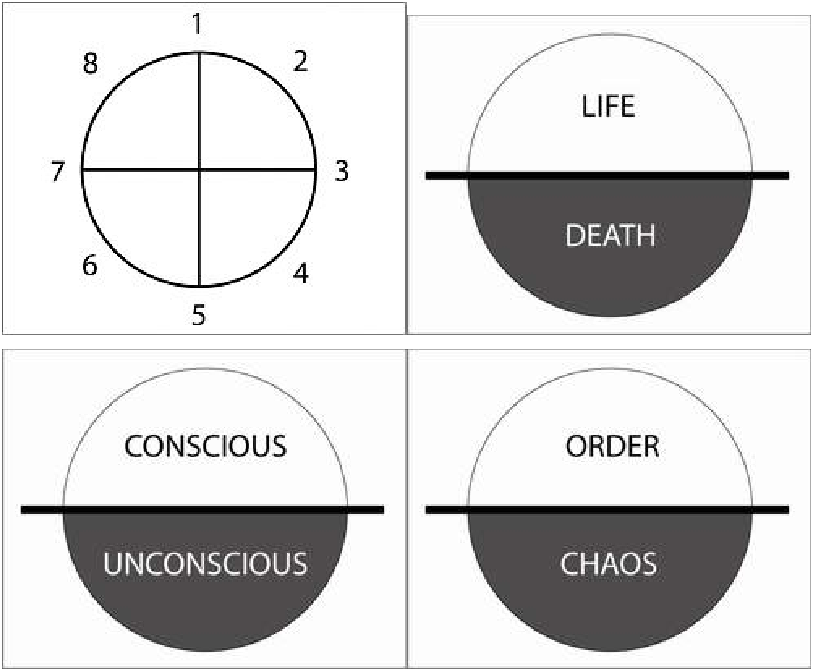
\includegraphics[width=0.48\textwidth]{figures/harmon02-all.pdf}
  \caption[]{
    Harmon cycles.
  }
  \label{fig:harmon-four}
\end{figure}

\begin{figure}[tbp!]
  \centering
  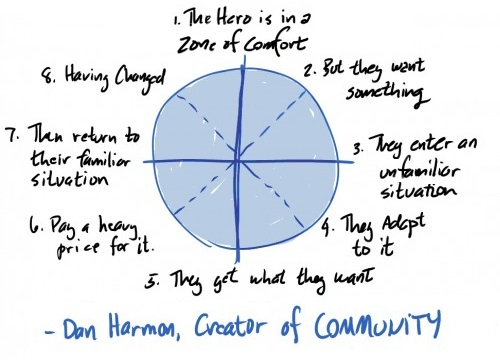
\includegraphics[width=0.48\textwidth]{figures/harmon05.jpg}
  \caption[]{
    Harmon cycles labeled.
  }
  \label{fig:harmon-labeled}
\end{figure}

\subsection{Papers}

A Bayesian Mixed Effects Model of Literary Character \cite{bamman2014bayesian}.

Culturally Based Story Understanding \cite{awad2013culturally}.

Persuasive Stories for Multi-Agent Argumentation \cite{bex2010persuasive}.

Values as the point of a story \cite{bex2013values}.

The Media Frames Corpus: Annotations of Frames Across Issues \cite{card2015media}.

Classifying temporal relations between events \cite{chambers2007classifying}.

Unsupervised Learning of Narrative Event Chains \cite{chambers2008unsupervised}..

Unsupervised learning of narrative schemas and their participants \cite{chambers2009unsupervised}.

A Database of Narrative Schemas \cite{chambers2010database}.

Event Schema Induction with a Probabilistic Entity-Driven Model \cite{chambers2013event}.

Learning Statistical Scripts with LSTM Recurrent Neural Networks \cite{pichotta2015learning}.

Novel Devotions: Conversional Reading, Computational Modeling, and the Modern Novel \cite{piper2015novel}.

\begin{quote}
  Use an LSTM on the narrative cloze dataset.
\end{quote}

Extracting social networks from literary fiction \cite{elson2010extracting}.
\begin{quote}
  We present a method for extracting social networks from literature, namely, nineteenth-century British novels and serials. We derive the networks from dialogue interactions, and thus our method depends on the ability to determine when two characters are in conversation. Our approach involves character name chunking, quoted speech attribution and conversation detection given the set of quotes. We extract features from the social networks and examine their correlation with one another, as well as with metadata such as the novel’s setting. Our results provide evidence that the majority of novels in this time period do not fit two characterizations provided by literacy scholars. Instead, our results suggest an alternative explanation for differences in social networks.
\end{quote}

Toward Automatic Character Identification in Unannotated Narrative Text \cite{valls2014toward}.
\begin{quote}
  An improvement in character detection is realized on a small set of stories by using feature-vectors around entities, built from POS of sentence parse tree.
\end{quote}

Toward Automatic Role Identification in Unannotated Folk Tales \cite{valls2014toward}.
\begin{quote}
  Uses ``action matrices''.
\end{quote}

\cite{collier2011understanding}
\cite{gelman2014stories}
\cite{bovet2016predicting}
\cite{mahoney2006tale}
\cite{levy2008case}
\cite{reece2016forecasting}


Learning Script Knowledge with Web Experiments \cite{regneri2010learning}.
\begin{quote}
  We describe a novel approach to unsupervised learning of the events that make up a script, along with constraints on their temporal ordering. We collect naturallanguage descriptions of script-specific event sequences from volunteers over the Internet. Then we compute a graph representation of the script’s temporal structure using a multiple sequence alignment algorithm. The evaluation of our system shows that we outperform two informed baselines.
\end{quote}

Minimally supervised event causality identification \cite{do2011minimally}.
\begin{quote}
  This paper develops a minimally supervised approach, based on focused distributional similarity methods and discourse connectives, for identifying of causality relations between events in context. While it has been shown that distributional similarity can help identifying causality, we observe that discourse connectives and the particular discourse relation they evoke in context provide additional information towards determining causality between events. We show that combining discourse relation predictions and distributional similarity methods in a global inference procedure provides additional improvements towards determining event causality.
\end{quote}

Learning to tell tales: a data-driven approach to story generation \cite{mcintyre2009learning}.
\begin{quote}
  Computational story telling has sparked great interest in artificial intelligence, partly because of its relevance to educational and gaming applications. Traditionally, story generators rely on a large repository of background knowledge containing information about the story plot and its characters. This information is detailed and usually hand crafted. In this paper we propose a data-driven approach for generating short children’s stories that does not require extensive manual involvement. We create an end-to-end system that realizes the various components of the generation pipeline stochastically. Our system follows a generate-and-and-rank approach where the space of multiple candidate stories is pruned by considering whether they are plausible, interesting, and coherent.
\end{quote}

Plot Induction and Evolutionary Search for Story Generation \cite{mcintyre2010plot}.
\begin{quote}
  In this paper we develop a story generator that leverages knowledge inherent in corpora without requiring extensive manual involvement. A key feature in our approach is the reliance on a story planner which we acquire automatically by recording events, their participants, and their precedence relationships in a training corpus. Contrary to previous work our system does not follow a generate-and-rank architecture. Instead, we employ evolutionary search techniques to explore the space of possible stories which we argue are well suited to the story generation task. Experiments on generating simple children’s stories show that our system outperforms previous data-driven approaches.
\end{quote}

Probabilistic Frame Induction \cite{cheung2013probabilistic}.
\begin{quote}
  In natural-language discourse, related events tend to appear near each other to describe a larger scenario. Such structures can be formalized by the notion of a frame (a.k.a. template), which comprises a set of related events and prototypical participants and event transitions. Identifying frames is a prerequisite for information extraction and natural language generation, and is usually done manually. Methods for inducing frames have been proposed recently, but they typically use ad hoc procedures and are difficult to diagnose or extend. In this paper, we propose the first probabilistic approach to frame induction, which incorporates frames, events, participants as latent topics and learns those frame and event transitions that best explain the text. The number of frames is inferred by a novel application of a split-merge method from syntactic parsing. In end-to-end evaluations from text to induced frames and extracted facts, our method produced state-of-the-art results while substantially reducing engineering effort.
\end{quote}

Learning Latent Personas of Film Characters \cite{bamman2014learning}.
\begin{quote}
  We present two latent variable models for learning character types, or personas, in film, in which a persona is defined as a set of mixtures over latent lexical classes.
  These lexical classes capture the stereotypical actions of which a character is the agent and patient, as well as attributes by which they are described.
  As the first attempt to solve this problem explicitly, we also present a new dataset for the text-driven analysis of film, along with a benchmark testbed to help drive future work in this area.
\end{quote}

Detecting Story Analogies from Annotations of Time, Action and Agency \cite{elson2012detecting}.
\begin{quote}
  We describe the Story Intention Graph (SIG) as a model of narrative meaning that is amenable to both corpus annotation and computational inference. The relations, focusing on time, action and agency, can express a range of thematic scenarios and lend themselves to the automatic detection of story similarity and analogy. An evaluation finds that such detection outperforms a propositional similarity metric in predicting human judgments of story similarity in the Aesop domain.
\end{quote}

Modeling Narrative Discourse \cite{elson2012modeling}.
\begin{quote}
  This thesis describes new approaches to the formal modeling of narrative discourse. Although
  narratives of all kinds are ubiquitous in daily life, contemporary text processing
  techniques typically do not leverage the aspects that separate narrative from expository
  discourse. We describe two approaches to the problem. The first approach considers the
  conversational networks to be found in literary fiction as a key aspect of discourse coherence;
  by isolating and analyzing these networks, we are able to comment on longstanding
  literary theories. The second approach proposes a new set of discourse relations that are
  specific to narrative. By focusing on certain key aspects, such as agentive characters, goals,
  plans, beliefs, and time, these relations represent a theory-of-mind interpretation of a text.
  We show that these discourse relations are expressive, formal, robust, and through the use
  of a software system, amenable to corpus collection projects through the use of trained
  annotators. We have procured and released a collection of over 100 encodings, covering
  a set of fables as well as longer texts including literary fiction and epic poetry. We are
  able to inferentially find similarities and analogies between encoded stories based on the
  proposed relations, and an evaluation of this technique shows that human raters prefer such
  a measure of similarity to a more traditional one based on the semantic distances between
  story propositions.
\end{quote}

Learning Narrative Structure from Annotated Folktales \cite{finlayson2011learning}.
\begin{quote}
  Narrative structure is an ubiquitous and intriguing phenomenon. By virtue of structure we recognize the presence of Villainy or Revenge in a story, even if that word is not actually present in the text.
  Narrative structure is an anvil for forging new artificial intelligence and machine learning techniques, and is a window into abstraction and conceptual learning as well as into culture and its influence on cognition. I advance our understanding of narrative structure by describing Analogical Story Merging (ASM), a new machine learning algorithm that can extract culturally-relevant plot patterns from sets of folktales. I demonstrate that ASM can learn a substantive portion of Vladimir Propp’s influential theory of the structure of folktale plots.
  The challenge was to take descriptions at one semantic level, namely, an event timeline as described in folktales, and abstract to the next higher level: structures such as Villainy, StuggleVictory, and Reward. ASM is based on Bayesian Model Merging, a technique for learning regular grammars. I demonstrate that, despite ASM’s large search space, a carefully-tuned prior allows the algorithm to converge, and furthermore it reproduces Propp’s categories with a chance-adjusted Rand index of 0.511 to 0.714. Three important categories are identified with F-measures above 0.8.
  The data are 15 Russian folktales, comprising 18,862 words, a subset of Propp’s original tales.
  This subset was annotated for 18 aspects of meaning by 12 annotators using the Story Workbench, a general text-annotation tool I developed for this work. Each aspect was doubly-annotated and adjudicated at inter-annotator F-measures that cluster around 0.7 to 0.8. It is the largest, most deeply-annotated narrative corpus assembled to date.
  The work has significance far beyond folktales. First, it points the way toward important applications in many domains, including information retrieval, persuasion and negotiation, natural language understanding and generation, and computational creativity. Second, abstraction from natural language semantics is a skill that underlies many cognitive tasks, and so this work provides insight into those processes. Finally, the work opens the door to a computational understanding of cultural influences on cognition and understanding cultural differences as captured in stories
\end{quote}

Crowdsourcing Narrative Intelligence \cite{li2012crowdsourcing}.
\begin{quote}
  Narrative intelligence is an important part of human cognition, especially in sensemaking and communicating with people. Humans draw on a lifetime of relevant experiences to explain stories, to tell stories, and to help choose the most appropriate actions in real-life settings. Manual authoring the required knowledge presents a significant bottleneck in the creation of systems demonstrating narrative intelligence. In this paper, we describe a novel technique for automatically learning script-like narrative knowledge from crowdsourcing. By leveraging human workers’ collective understanding of social and procedural constructs, we can learn a potentially unlimited range of scripts regarding how real-world situations unfold. We present quantitative evaluations of the learned primitive events and the temporal ordering of events, which suggest we can identify orderings between events with high accuracy.
\end{quote}


Computational Narrative Intelligence: A Human-Centered Goal for Artificial Intelligence \cite{riedl2016computational}.
\begin{quote}
  Narrative intelligence is the ability to craft, tell, understand, and respond affectively to stories. We argue that instilling artificial intelligences with computational narrative intelligence affords a number of applications beneficial to humans. We lay out some of the machine learning challenges necessary to solve to achieve computational narrative intelligence. Finally, we argue that computational narrative is a practical step towards machine enculturation, the teaching of sociocultural values to machines.
\end{quote}


A computational model for plot units \cite{goyal2013computational}.
\begin{quote}
  This research revisits plot units, which were developed in the 1980s as a conceptual knowledge structure to represent the affect states of and emotional tensions between characters in narrative stories. We present a fully automated system, called AESOP, that generates plot unit representations for narrative texts. AESOP performs four steps: affect state recognition, character identification, affect state projection, and link creation. We also identify a type of knowledge that seems to be missing from existing lexical resources: verbs that impart positive or negative polarity onto their patients (e.g., “eat” imparts negative polarity because being eaten is bad, whereas “fed” imparts positive polarity because being fed is good). We develop two techniques to automatically harvest these “patient polarity verbs” (PPVs) from a Web corpus, and show that the PPVs improve affect state recognition. Finally, we evaluate AESOP’s performance on a set of fables, and present several analyses to shed light on the capabilities and limitations of current natural language processing technology for plot unit generation.
\end{quote}


Computational approaches to figurative language \cite{shutova2011computational}.
\begin{quote}
  I adopt a statistical data-driven approach to its modelling, and create the first open-domain system for metaphor identification and interpretation in unrestricted text. In order to verify that similar methods can be applied to modelling other types of figurative language, I then extend this work to the task of interpretation of logical metonymy.
\end{quote}


\subsection{Story graphs, plot diagrams, and inferring causality}

With the distinction between plot, structure, and emotional trajectory in mind, there have also been attempts to discover plot using data driven methods.
Using topic modeling, both \cite{schmidt2015plot} and \cite{jockers2013macroanalysis} find known patterns of plot across many thousand stories.
In \cite{piper2015novel}, computational analysis is applied to realize the potential of distant reading (see \cite{moretti2013distant}) to find and test scholarly insights.
In \cite{winston2011strong}, a system called ``Genesis'' is developed to compare plot summaries using casual connections between events, laid out as a the \textit{Strong Story Hypothesis}:
\begin{quote}
  The mechanisms that enable humans to tell, understand, and recombine stories separate human intelligence from that of other primates.
\end{quote}

The next wave of NLP advances that aim to decode stories may very well be a breakthrough in understanding human nature \cite{cambria2014jumping}.

\subsection{Character Networks}

An Interactive Visualization of Every Line in Hamilton
Shirley Wu
http://polygraph.cool/hamilton/



\subsection{Emotional arcs}

With the same goals in pursuing the story shapes first elaborated by \cite{vonnegut1981palm}, in a series of blog posts \cite{jockers2016novel} lays out a strategy for generating emotional arcs and eventually finds six story types using hierarchical clustering.
Our work in Chapter 3 is an continuation of a very different core methodology that we first propose in \cite{dodds2015human}.
As we note in Chapter 3 as well, the distinction between plot and emotional arc, as well as using sentiment analysis tools correctly distinguish our contributions from those of \cite{jockers2016novel}.

\subsection{Debates in the digital humanities}

\textit{Validity} by David Bamman (\href{http://www.davidbamman.com/?p=52}{http://www.davidbamman.com/?p=52}).

\textit{Not Enough Perspectives, Pt. 1} by Scott Weingart (\href{http://www.scottbot.net/HIAL/index.html@p=41271.html}{http://www.scottbot.net/HIAL/index.html@p=41271.html}).

\textit{Man in Hole II: Man in Deeper Hole} by Dan Piepenbring (\href{http://www.theparisreview.org/blog/2015/03/19/man-in-hole-ii-man-in-deeper-hole/}{http://www.theparisreview.org/blog/2015/03/19/man-in-hole-ii-man-in-deeper-hole/}).
%% March 19, 2015, The Paris Review

\textit{Validation and Subjective Computing} by Andrew Piper (\href{http://txtlab.org/?p=470}{http://txtlab.org/?p=470}).

\textit{A Fabula of Syuzhet: A Contretemps of Digital Humanities and Sentiment Analysis} by Eileen Clancy (\href{https://storify.com/clancynewyork/contretemps-a-syuzhet}{https://storify.com/clancynewyork/contretemps-a-syuzhet}).
%% 11 months ago

\textit{Plot arceology 2016: emotion and tension} by Ben Schmidt (\href{http://sappingattention.blogspot.com/2016/07/plot-arceology-emotion-and-tension.html}{http://sappingattention.blogspot.com/2016/07/plot-arceology-emotion-and-tension.html}).

Tragedy:
http://hedonometer.org/books/v3/154/?lens=[3,7]
http://hedonometer.org/books/v3/2413/?lens=[3,7]
Rags to riches:
http://hedonometer.org/books/v3/5348/?lens=[3,7]

Using the jocker's approach here, Julia Silge appears to have stolen it. (No reference to Jockers).
http://juliasilge.com/blog/If-I-Loved-NLP-Less/
And here
http://nacnudus.github.io/crossprod/harry-potter-and-the-n-grams-of-sentiment
Here:
https://duncan-garmonsway.shinyapps.io/harry-potter/
And then they find ours:
http://nacnudus.github.io/crossprod/more-harry-potter-story-arcs-they-get-darker
